 ---------------------------------------------------------------------
% ---------------------------------------------------------------------
% ---------------------------------------------------------------------

\chapter{Fonaments del reconeixement automàtic de la parla}
\label{cap02__}

% ---------------------------------------------------------------------
% ---------------------------------------------------------------------
% ---------------------------------------------------------------------

Aquest capítol proporciona els coneixements teòrics necessaris per entendre el treball realitzat. S'estructura de la següent manera: 
primer, la Secció~\ref{cap02_reconeixement_patrons} defineix els conceptes i les bases matemàtiques del reconeixement de formes. 
Després, la Secció~\ref{cap02_aprenentatge_maquina} dona unes nocions bàsiques sobre l'aprenentatge automàtic, així com els principals reptes i algunes tècniques utilitzades.
A continuació, la Secció~\ref{cap02_xarxes_neuronals} explica les diferents arquitectures de xarxes neuronals que solen gastar-se en el desenvolupament de sistemes híbrids d'ASR.
Finalment, la Secció~\ref{cap02_recon_autom_parla} detalla el desenvolupament d'un sistema ASR híbrid i dels seus components, així com la forma d'avaluar-los.

\section{Reconeixement de formes}
\label{cap02_reconeixement_patrons}

El Reconeixement de Formes (Pattern Recognition) és una aproximació a la classificació de dades que, de forma automàtica i mitjançant algorismes, pretén extraure la informació que permeta establir propietats o característiques amb les que classificar aquestes dades.
En aquest context, trobem tres conceptes bàsics:
\begin{itemize}
    \item \emph{Classe}: aquest concepte representa a un grup de dades que comparteixen característiques similars. Un exemple clàssic de reconeixement de formes és el de dues classes diferents en les quals podem classificar un correu electrònic: \emph{spam} i \emph{no-spam}, que indiquen, respectivament, si el contingut d'un missatge es o no considerat spam per a l'usuari.
    
    \item \emph{Objecte}: un objecte es una instància d'una classe, que típicament fa referència a un vector $\textbf{x} \in \mathbb{R}^D$, que representa un conjunt de característiques mesurables, extretes de l'objecte en qüestió, i $D$ el número de característiques considerades, que defineix la dimensionalitat del problema.
    Un exemple clàssic és el de classificar flors de la família \textit{Iris} en tres classes: \emph{setosa}, \emph{versicolor} i \emph{virgínica}, on, per exemple, s'usen les dimensions (altura i amplària) dels pètals i dels sèpals com a característiques.
    D'aquesta manera treballem en un espai 4-dimensional, amb objectes representats per quatre dimensions: altura del pètal, amplària del pètal, altura del sèpal, i amplària del sèpal.
    
    \item \emph{Classificació}: classificar un objecte consisteix en seleccionar la classe a la qual tinga major probabilitat de pertànyer d'acord amb una regla de decisió. Aquesta regla apareix a l'aplicar una funció $f \colon \textbf{x} \to c \in C$, on $\textbf{x}$ és l'objecte a classificar, $c$ és l'etiqueta de classe assignada a l'objecte $\textbf{x}$ segons $f$, i $C$ és el set de classes del problema.
\end{itemize}

S'ha mencionat en diverses ocasions el vector de característiques, aquell que conté la informació que representa a un objecte. La tasca d'establir aquests vectors s'anomena extracció de característiques, i és un dels passos inicials.
Aquest processat per al cas del reconeixement automàtic de la parla està degudament explicat en la Secció \ref{cap02_preprocessat_acustic}.

Quan es parla de classificació estadística, la funció que proporciona informació per decidir a quina classe $c$ pertany un objecte $x$ és un model probabilístic $P(c|x)$. Aquesta funció està relacionada amb el teorema de Bayes:

\begin{equation}\label{eq:teor_bayes}
    P(c \mid \textbf{x}) = \frac{P(\textbf{x} \mid c) \, P(c)}{P(\textbf{x})}
\end{equation}

Aplicant aquesta fórmula podem conéixer a quina classe $c$ té més probabilitats de pertànyer un objecte $\textbf{x}$. A aquesta classe, que maximitza la probabilitat ``a posteriori'' de la classe $P(c \mid \textbf{x})$, se la denota com $\hat{c}$:

\begin{equation}\label{eq:form_argmax_classif}
    \hat{c} = \argmax_{c \in C} P(c \mid \textbf{x}) = \argmax_{c \in C} \frac{P(\textbf{x} \mid c) \, P(c)}{P(\textbf{x})}
\end{equation}

Donat que $P(\textbf{x})$ és constant per a tota classe $c \in C$, podem simplificar l'equació d'aquesta manera:

\begin{equation}\label{eq:form_argmax_classif_simpli}
	\hat{c} = \argmax_{c \in C} P(\textbf{x} \mid c) \, P(c)
\end{equation}

D'aquesta manera i, en funció de la tasca de Pattern Recognition a desenvolupar, es pot optar per modelar directament $P(c|\textbf{x})$, o bé per modelar separadament $P(\textbf{x} \mid c)$ i $P(c)$.
Les tècniques que s'usen per modelar cadascuna d'eixes probabilitats dependran igualment del tipus de tasca.


% ----------------------------------------------------------------------------------------
% ----------------------------------------- ¿  ? -----------------------------------------
% ----------------------------------------------------------------------------------------
\section{Aprenentatge automàtic}
\label{cap02_aprenentatge_maquina}

L'aprenentatge automàtic (Machine Learning), és el camp de la inte\lgem ència artificial que es dedica a l'estudi i desenvolupament d'algorismes i tècniques amb la capacitat de \textbf{generalitzar} un tipus de problema i \textbf{aprendre} a resoldre'l de forma autònoma.
Generalitzar és, en aquest context, tindre la capacitat d'actuar de manera adequada davant de dades noves, que no s'han presentat prèviament. 
Per tant, podem dir que l'aprenentatge automàtic és l'àrea que s'encarrega d'estudiar la millor manera de parametritzar i d'aproximar models probabilístics de l'equació~\ref{eq:form_argmax_classif_simpli}.

Una definició de què és ``aprendre'' en aquest camp li la devem a Tom Mitchell\cite{mit97machinelearning}:\\
\guillemotleft Es diu que un programa pot aprendre d'una experiència $E$ respecte a un conjunt de tasques $T$ i la mesura de rendiment $P$, si el seu rendiment a les tasques de $T$, mesurat per $P$, millora amb l'experiència $E$\guillemotright.

Podem classificar aquestes tècniques i algorismes en tres grans branques o categories bàsiques:

\begin{itemize}
    \item \textbf{Aprenentatge supervisat}: aquesta tècnica intenta induir una funció $f$ similar a les vistes anteriorment, que assigna a cada valor d'entrada $x$, un valor d'eixida $c$, basant-se en una co\lgem ecció de parells d'exemples entrada-eixida.
    És a dir, donat un conjunt d'$N$ parells de mostres d'entrenament, $(x_1, c_1), (x_2, c_2), \dots (x_N, c_N)$, on cada parell ha sigut generat per una funció desconeguda $c_n = f(x_n)$, el sistema intenta descobrir, o generar, una funció $\hat{f}$ que s'aproxime el màxim possible a la funció $f$ desconeguda.
    Per la seua naturalesa són emprades en tota mena de tasques de regressió i classificació, on els valors d'eixida són numèrics o etiquetes de classe, respectivament.

    \item \textbf{Aprenentatge no supervisat}: aconseguir suficients quantitats de dades etiquetades és, en moltes ocasions, una tasca molt costosa. L'aprenentatge no supervisat no usa coneixement \textit{a priori}\footnote{Coneixement que no prové de l'experiència, en el nostre cas és preassignat per un coneixement expert.}, tracta al conjunt de dades com a variables aleatòries i extrau patrons ocults d'elles.
    Per tant, aquests algorismes tenen la capacitat d'identificar característiques sense ajuda externa i, posteriorment, relacionar els objectes per a classificar-los, etiquetar-los i d'agrupar-los.

    \item \textbf{Aprenentatge per reforç}: la característica principal és que no aprén mitjançant un conjunt de dades, el sistema aprén interaccionant amb l'entorn.
    El sistema controla a un \emph{agent}, que pot ser real o simulat, capaç d'interactuar amb el seu entorn, també real o simulat. Quan l'agent realitza una acció se li recompensa amb un valor, que pot ser positiu o negatiu, directament relacionat amb l'estat actual, que afegirà al \textit{retorn} (recompensa acumulada).
    L'algorisme intenta maximitzar el \textit{retorn}. Açò comporta l'aprenentatge de rutines i comportaments que permeten al sistema obtenir un gran rendiment en la seua tasca.
\end{itemize}

Per a més informació sobre tècniques d'aprenentatge automàtic, es remet la lectora a~\cite{russell2020artificial}.

La forma en què s'entrenen aquests sistemes, així com les dades emprades poden tindre també una influència nefasta en el seu rendiment. Els principals reptes que aquestes tècniques presenten són els següents:
\begin{itemize}
    \item \textbf{Sobreajustament (overfitting)}: l'objectiu de l'aprenentatge automàtic és generalitzar un problema d'acord amb unes dades d'entrenament. 
    Hi ha determinades tècniques que, si no s'ajusten amb cura, poden provocar l'efecte contrari: es ``memoritza'' el conjunt d'entrenament. És a dir, els paràmetres del sistema o model entrenat s'ajusten tant acuradament a les dades d'entrenament que deixen de tindre cap sentit fora del conjunt d'entrenament. 
    D'aquesta manera el model comet errors significatius al processar dades no vistes en entrenament, i no és útil per al seu propòsit.

    \item \textbf{Parcialitat (biaix algorítmic)}: quan s'entrena un model estadístic amb unes dades que no representen correctament la població real (siga per falta de dades, per mala elecció d'aquestes, o perquè són corruptes/errònies), determinats algorismes i models aprenen a donar prioritat a unes classes sobre altres que no eren les esperades.
    Açò pot donar lloc a molts problemes quan el sistema ha de tractar amb persones, ja que pot presentar discriminació de gènere\cite{bias_gender_discrim}, raça\cite{bias_racial_discrim} i inclús discriminació sexual\cite{bias_sexual_discrim}.
\end{itemize}

A continuació s'exposen algunes tècniques que facilitaran la comprensió dels subsegüents apartats.

\subsection{Arbres de classificació}
Els arbres de classificació i regressió (CART, Classification and Regression Trees) són un tipus d'algorisme que classifica les dades en un arbre de decisions mitjançant preguntes tancades binàries (Sí/No). D'aquesta manera, després és molt senzill explorar-lo i obtenir els conjunts de dades pertinents.

Durant la creació de l'arbre s'intenta que les particions siguen tan homogènies com siga possible. Per a aconseguir-ho, s'avaluen les diferents preguntes possibles mitjançant la impuresa de Gini, així la partició que tinga la impuresa més baixa serà l'elegida.
La divisió òptima es realitza de forma iterativa fins a arribar a unes condicions concretes de dades mínimes a la branca o una impuresa màxima.

Per a més informació sobre els algorismes CART, es recomana la lectura de \cite[cap. 18.1]{pml1Book}.

\subsection{Models de mixtures de Gaussianes}
\label{cap02_mixtures}
La clusterització de dades és una tècnica d'aprenentatge no supervisat molt comú a l'aprenentatge màquina (agrupacions) que intenta trobar conjunts de dades amb característiques en comú.

Un model de mixtura de Gaussianes (GMM, Gaussian Mixture Model) és una funció composada per $K$ Gaussianes, on $K$ típicament és el nombre de classes del problema, ja que cada component (Gaussiana) s'especialitza en explicar els objectes de la seua classe. Cada Gaussiana, $k$, és una funció que conté els següents paràmetres:

\begin{itemize}
    \item La mitjana, $\mu_k$, que defineix el seu centre.
    \item La variància, $\Sigma_k$, que defineix la seua amplària.
    \item El pes, $\pi_k$, que indica quantes dades estan associades a la Gaussiana sobre el total (tant per un). Com que hi ha una gaussiana per a cada classe, tenim que $\sum_{k=1}^K \pi_k = 1$.
\end{itemize}

Per a aconseguir que cada Gaussiana s'especialitze en una classe diferent es segueix l'algorisme Expectation-Maximisation~\cite{10.2307/2984875}:

\begin{enumerate}
    \item Inicialització de les Gaussianes de forma aleatòria, o bé amb el resultat d'un agrupament per \textit{K-Means}~\cite{JAIN2010651}.
    \item Fins a convergència de l'algorisme (no hi ha canvis en els agrupaments):
        \begin{enumerate}[label=(\arabic*)]
            \item Assignació de dades a cada Gaussiana per proximitat.
            \item Recalcular paràmetres de cada Gaussiana amb les noves dades assignades.
        \end{enumerate}
\end{enumerate}

Per ampliar coneixements sobre les GMM es recomana a la lectora la lectura de~\cite[Capítol 2.5]{jurafskySLP}.

% ----------------------------------------------------------------------------------------
% ----------------------------------------- ¿  ? -----------------------------------------
% ----------------------------------------------------------------------------------------
\section{Xarxes neuronals}
\label{cap02_xarxes_neuronals}
Una xarxa neuronal, o xarxa neuronal artificial, és un conjunt d'estructures processadores densament connectades.
Les estructures reben el nom de \textit{neurones}, estan dividides en diferents capes i diem que estan densament connectades perquè cada neurona d'una capa està connectada a totes les neurones de la capa següent. 
Una xarxa neuronal té com a mínim tres capes diferents: una capa d'entrada rep les dades, una o múltiples capes ocultes que realitzen diferents projeccions lineals i no lineals sobre les dades d'entrada i càlculs interns parcials, i la capa d'eixida que retorna la informació processada, bé en forma d'objecte (regressió), o bé en forma de predicció d'etiquetes de classe (classificació).

A les capes ocultes i a la d'eixida, cada neurona, realitza el processat seguint la següent fórmula:

\begin{equation}
y(\textbf{x}, \textbf{w}) = f \Big( \sum_{j=1}^M w_j \phi_j(\textbf{x}) \Big)
\label{eq:prob_neurona}
\end{equation}
on $f$ es la \textit{funció d'activació}, que s'aplica al valor de retorn de la neurona, generalment per introduir transformacions no lineals, $w_j$ són els paràmetres (pesos) que connecten la neurona i-èsima amb les de la capa anterior, $\phi_j(\textbf{x})$ és l'eixida de la capa anterior i $M$ és el nombre de neurones en la capa actual.
Aquest model bàsic de xarxa neuronal, on la informació que genera una capa flueix estrictament a la capa posterior, rep el nom de xarxa neuronal profunda directa (FF-DNN). 
La figura~\ref{fig:estructura_fnn} mostra una possible estructura de FF-DNN.

\begin{figure}[ht!]
    \centering
    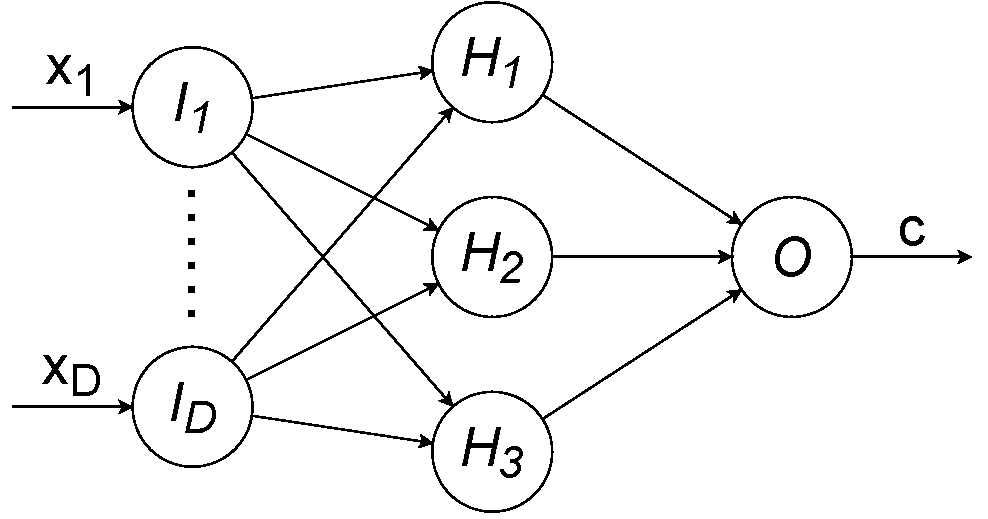
\includegraphics[width=0.5\textwidth]{figuras/estructura_fnn.pdf}
    \caption{Exemple d'estructura d'una xarxa neuronal profunda directa de tres capes: una d'entrada, una oculta i una d'eixida. Cada neurona $n_j$ està connectada amb totes les neurones de la capa posterior $n_{j+1}$.}
    \label{fig:estructura_fnn}
\end{figure}

La funció d'activació, a més d'assignar un valor d'eixida en un rang, apareix per la necessitat d'usar les neurones de forma selectiva, activant les adequades i no actualitzant altres, cosa que permet treballar amb dades no separables linealment.

A continuació es presenten algunes funcions d'activació interessants, així com una petita descripció de cada una:
\begin{itemize}
    \item Sigmoid: es defineix com $f(x)=\frac{1}{1+e^{-x}}$. És senzilla i té un cost temporal baix; el problema més gros és que la derivada genera ràpidament pèrdua d'informació, el que es coneix com a \textit{problema d'esvaïment de gradient}, que no permet a les primeres capes de la xarxa aprendre informació important quan es fa la \textit{retropropagació} (explicada adequadament a continuació).
    \item Tangent hiperbòlica: s'expressa com $f=\frac{e^x-e^{-x}}{e^x+e^{-x}}$, sent el seu rang d'eixida $[-1, 1]$. És típicament preferida sobre la funció Sigmoid, però no resol el problema d'esvaïment de gradient.
    \item ReLu (Rectified Linear Unit): aquesta funció extremadament simple, $f(x)=max(0, x)$, activa les neurones únicament per a valors d'entrada positius. A més, aconsegueix resoldre el problema d'esvaïment de gradient.
    \item Softmax: $f(x)=\frac{e^x}{\sum_i e^{x_i}}$ . Permet interpretar els valors d'eixida de la capa sobre la que s'aplica com una distribució de probabilitat. S'aplica típicament en la capa d'eixida en tasques de classificació.
\end{itemize}

La retropropagació (backpropagation), és l'algorisme que permet aprendre els pesos $w_j$ de l'equació~\ref{eq:prob_neurona} a partir d'un conjunt de dades d'entrenament, d'acord amb algun criteri d'optimització.
En primer lloc, es realitza una inferència cap endavant usant un lot (batch) de dades d'entrenament fins a la capa d'eixida. A continuació, es mesura la divergència entre els valors obtesos a la capa d'eixida i els valors esperats. Aquesta diferència es propaga cap enrere a través de les capes ocultes de la xarxa, modificant apropiadament els pesos de les neurones per minimitzar aquestes diferències. Aquest procés es repeteix de manera iterativa fins convergència. 
Més informació sobre l'algorisme de retropropagació es pot trobar a \cite{rumelhart1986backpropagation}.

Tal i com s'ha mencionat adés, les xarxes neuronals poden tindre més d'una capa oculta. 
Amb aquesta arquitectura, les capes més pròximes a la capa d'entrada aconsegueixen especialitzar-se en xicotets detalls, mentre que les capes més profundes s'especialitzen en característiques més generals i invariants. 
Gràcies a aquest augment de la complexitat i de la grandària d'aquestes xarxes, també ha augmentat la capacitat de processament sobre dades, i és que com s'ha demostrat~\cite{HORNIK1989359}, les DNN compleixen el teorema de l'aproximació universal, que en línies generals diu \guillemotleft Qualsevol funció pot ser \textbf{aproximada} per una xarxa neuronal amb una precisió $p$, tal que  $p < \epsilon$, sent $\epsilon$ un nombre real positiu pròxim a zero, si li proporcionem les suficients neurones\guillemotright. 
En conseqüència, la potència de computació necessària escala de manera proporcional.

\subsection{Xarxes neuronals recurrents}
En tasques com ASR es tracta el processament de seqüències temporals, els components de les quals tenen una gran interdependència interna.
Per exemple, en la producció del llenguatge natural, les seqüències de paraules tenen dependències d'ordre > 1; en la producció fonètica, les seqüències de fonemes també mostren una interdependència (no és el mateix pronunciar una /k/ abans d'una /a/ que d'una /e/, per exemple).
Mitjançant xarxes neuronals recurrents (RNN) és possible aprofitar aquesta informació contextual gràcies a les seues connexions cícliques, i és que les RNNs són, en essència, un tipus de xarxa neuronal amb cicles directes en les seues neurones, que donen lloc a una estructura d'estats interns o memòria~\cite{Yu2015AutomaticSR}.

Una de les arquitectures de xarxes RNN que més rellevància ha generat és la Long Short-Term Memory (LSTM)~\cite{hochreiter1997lstm}, que té com a unitat bàsica la ce\lgem a LSTM, l'encarregada de connectar informació passada a la tasca actual. Aquesta ce\lgem a està formada per tres tipus de portes: la d'entrada, que controla la informació que entra en la ce\lgem a, la de sortida, que controla la informació que ix d'ella i la porta d'oblit, que s'encarrega de recordar o oblidar la informació prèvia de la ce\lgem a. La figura~\ref{fig:estructura_lstm_cell} mostra l'estructura interna bàsica d'una ce\lgem a LSTM.
Per a una explicació més detallada sobre el funcionament d'una xarxa LSTM, es recomana la lectura de~\cite{colah2015lstm}.

\begin{figure}[ht!]
    \centering
    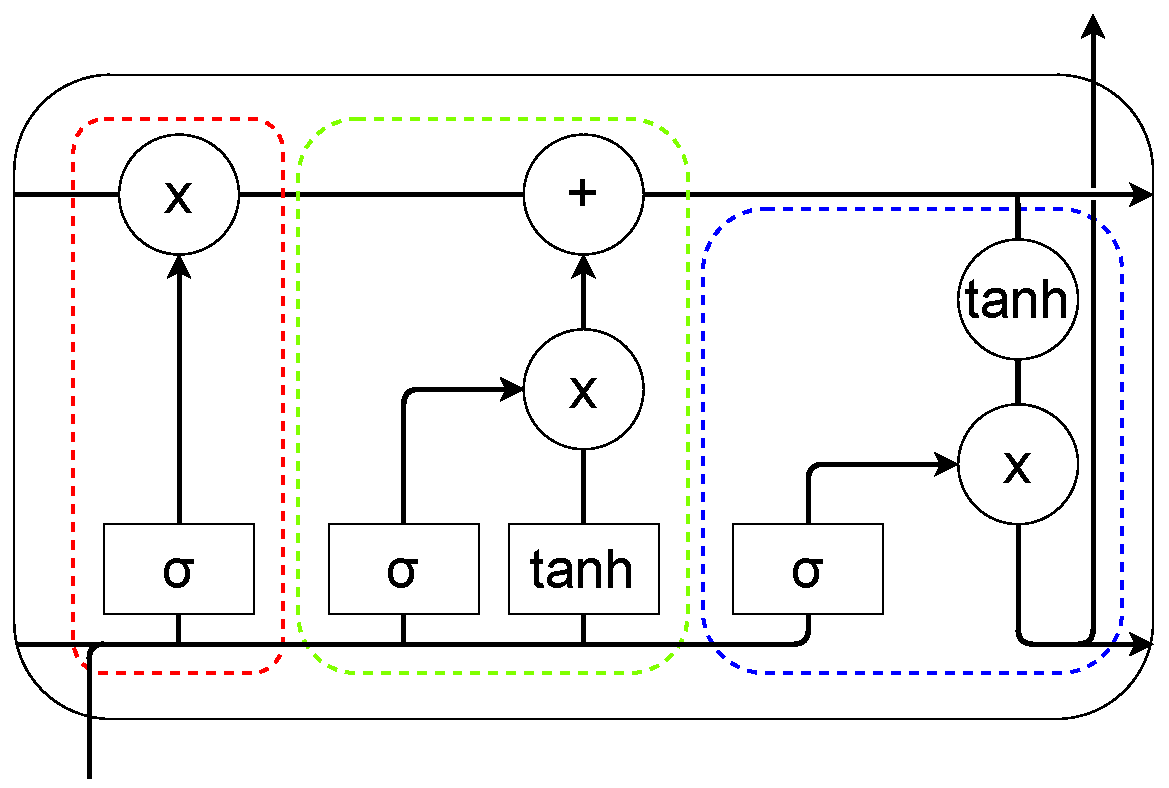
\includegraphics[width=0.8\textwidth]{figuras/estructura_lstm_cell.pdf}
    \caption{Estructura interna d'una ce\lgem a LSTM, on els cercles representen operacions a nivell d'elements, els rectangles representen una capa de xarxa neuronal amb una funció d'activació (sigmoid o $\tanh$). Dues fletxes unint-se representen concatenació de dades, mentre que la seua separació significa que el seu contingut s'envia a diferents localitzacions. L'àrea marcada en roig representa la porta d'oblit, la verda la d'entrada i la blava la de sortida.}
    \label{fig:estructura_lstm_cell}
\end{figure}

Una evolució lògica de les LSTMs son les LSTM bidireccionals (BLSTM), que permeten analitzar les dades en ambdós sentits temporals al mateix temps. Per a aconseguir-ho es duplica l'estructura prèvia, però començant per l'última dada i acabant per la primera. La figura~\ref{fig:lstm_vs_blstm} mostra una comparació visual de la bidireccionalitat aplicada a una xarxa amb la versió unidireccional d'aquesta.

\begin{figure}[ht!]
    \centering
    \begin{subfigure}{0.3\textwidth}
        \centering
        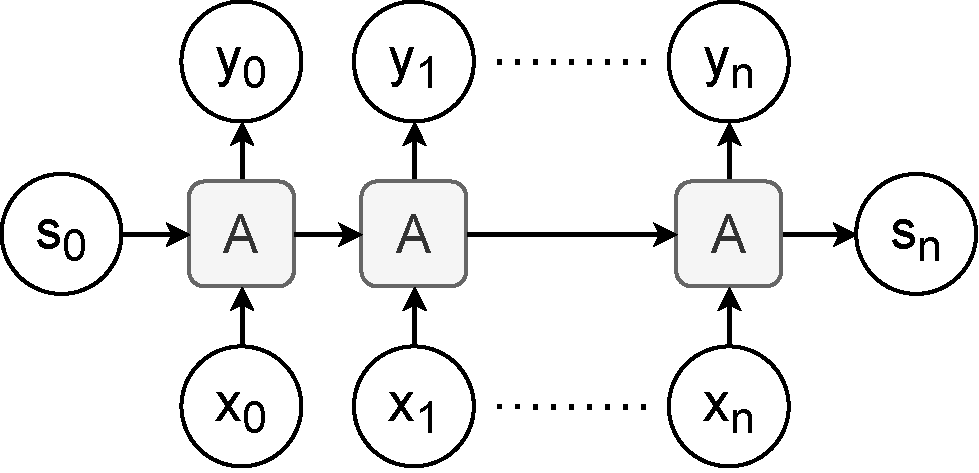
\includegraphics[width=\textwidth]{figuras/lstm_vs_blstm_a.pdf}
        \caption{Xarxa unidireccional}
    \end{subfigure}
    \hfill
    \begin{subfigure}{0.6\textwidth}
        \centering
        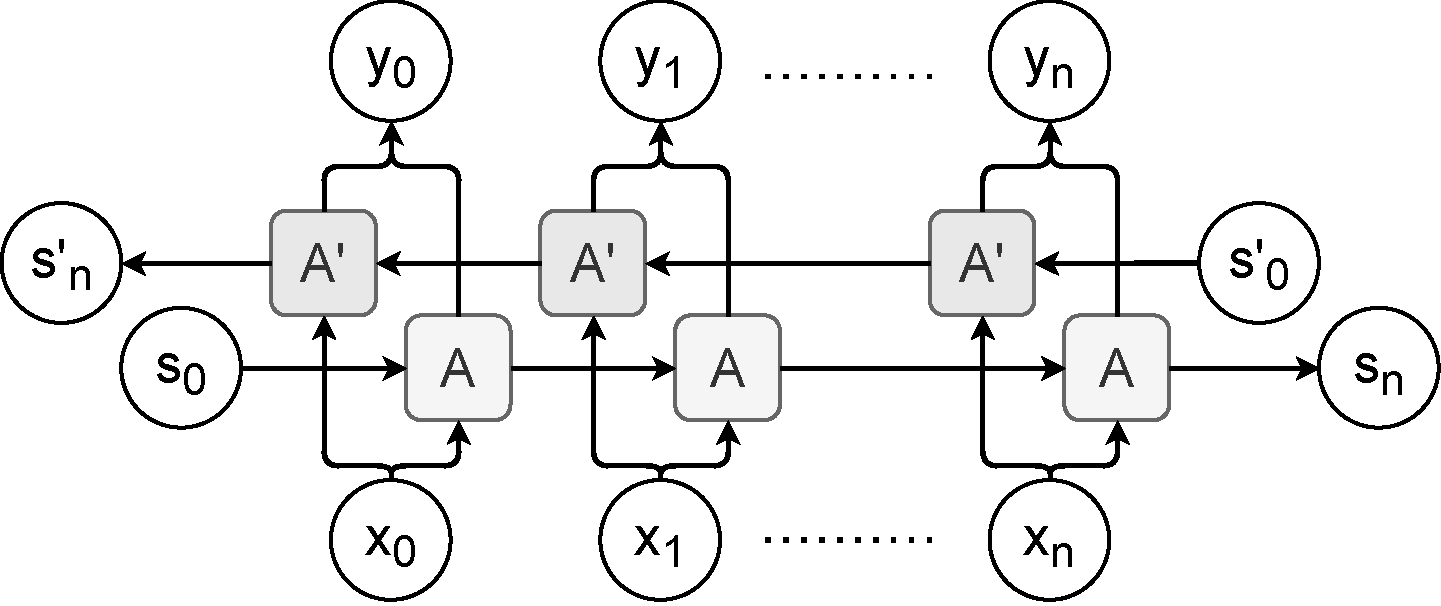
\includegraphics[width=\textwidth]{figuras/lstm_vs_blstm_b.pdf}
        \caption{Xarxa bidireccional}
    \end{subfigure}
    \caption{Comparativa entre una xarxa unidireccional (esquerra) i una altra bidireccional (dreta). A la xarxa bidireccional es pot observar com ambdós estats $s_0$ i $s'_0$ inicien les seues operacions als extrems contraris. Cada subestructura vertical formada pel component d'entrada $x_n$, el d'eixida $y_n$ i la ce\lgem a $A$, o ce\lgem és $A$ i $A'$, és una representació de la xarxa a l'instant $n$.}
    \label{fig:lstm_vs_blstm}
\end{figure}



\subsection{Arquitectura Transformer}

En els últims anys, l'arquitectura Transformer, basada en el concepte d'auto-atenció~\cite{vaswani2017transformers}, s'ha posicionat com l'arquitectura d'avantguarda en múltiples tasques, especialment en el camp del modelat del llenguatge natural.
L'atenció, en aquest camp, és una tècnica que intenta imitar l'atenció cognitiva dels éssers vius, amb l'objectiu focalitzar-se en els conjunts de dades més importants.
Té una estructura encoder-decoder, que assigna seqüències de vectors d'entrada, $(\textbf{x}_1, \dots, \textbf{x}_n)$, a seqüències de vectors d'eixida, $(\textbf{y}_1, \dots, \textbf{y}_n)$, de la mateixa mida. En concret, cada capa està formada per un conjunt de subcapes que contenen xarxes neuronals totalment connectades.
Totes les seves característiques li concedeixen una sèrie d'avantatges front a un RNN: processament en para\lgem el de les dades (en lloc de seqüencial), possibilitat d'atendre potencialment a històries infinites gràcies al mecanisme de d'auto-atenció, entre altres.
Per més informació sobre aquesta arquitectura, remetem a la lectora a~\cite[capítol 9.7]{jurafskySLP}.




\section{Reconeixement automàtic de la parla}
\label{cap02_recon_autom_parla}

ASR és la tecnologia que dota a un sistema automàtic de la capacitat de, partint d'un discurs parlat, obtenir la seqüència de paraules més probable, $\hat{w}$, que la transcriu, mitjançant l'anàlisi de seqüències de vectors de característiques $\textbf{x}$ obtinguts en analitzar el senyal acústic.

Una primera aproximació és l'anomenada sequence-to-sequence, que tracta de modelar directament la probabilitat ``a posteriori'' $P(w | \textbf{x})$. 
El problema d'eixa aproximació és que per entrenar els models sols es poden usar dades de parla etiquetada, i això no és possible en tots els casos per mancança de dades, o bé per l'elevat cost d'etiquetatge d'aquest tipus de dades, especialment si l'etiquetatge és manual. 

L'alternativa són els sistemes híbrids, que opten per aplicar Bayes a la probabilitat a posteriori de la classe (veure Eq.~\ref{eq:form_argmax_classif}). D'aquesta manera, l'Equació~\ref{eq:form_argmax_classif_simpli} es redefineix com segueix:

\begin{equation}\label{eq:form_argmax_classif_ASR}
	\hat{w} = \argmax_{w \in L^{*}} P(w | \textbf{x}) = \argmax_{w \in L^{*}} P(\textbf{x} | w) \, P(w)
\end{equation}
sent $L$ el conjunt de paraules que pot reconèixer el sistema, i $L^{*}$ el conjunt de totes les possibles frases (seqüències de paraules) d'aquest llenguatge. $P(w)$, anomenat model del llenguatge (LM, Language Model), calcula la probabilitat que la frase $w$ forme part del llenguatge $L$, mentre que $P(\textbf{x} | w)$, anomenat model acústic (AM, Acoustic Model), calcula la probabilitat de que aquesta seqüència de paraules $w$ genere la seqüència de vectors acústics $\textbf{x}$.
El gran avantatge de l'aproximació híbrida és que el model del llenguatge es pot entrenar amb una font massiva de dades: text monolingüe en la llengua $L$. Això dona lloc a un component (LM) molt robust, potent i versàtil, i que contribueix de manera decisiva en la millora prestacional dels sistemes ASR. En aquest punt convé ressaltar que aquest treball està centrat en el desenvolupament de models acústics per a sistemes ASR híbrids.

Abans d'entrar en matèria d'algorismes, es contextualitza la dimensió de la problemàtica a resoldre. En primer lloc, la dimensió del vocabulari és clau, ja que influeix directament en la complexitat temporal i espacial del procés d'inferència, reconeixement o decoding, així com en la complexitat del model del llenguatge, que determina el vocabulari del sistema.
Hi ha models que s'entrenen per a reconéixer vocabularis xicotets (p.e. dígits, on hi ha 10 possibilitats) on és més senzill obtenir una gran precisió que en grans models on s'intenta modelar la conversa humana (centenars de milers de paraules).
També cal comentar el domini de les dades a transcriure, no és el mateix transcriure retransmissions esportives que conferències sobre física de partícules (CERN). El vocabulari i les dades d'entrenament poden ser més o menys adaptades a la tasca, i això influeix també en la qualitat del reconeixement.

En segon lloc, el soroll, la reverberació, l'equipament de captura, el nivell de compressió de l'àudio, i altres problemes acústics també dificulten el reconeixement, ja que en un espai amb silenci un micròfon professional s'aconseguirà una mostra de major qualitat que un àudio enregistrat en una revetlla d'estiu amb el telèfon mòbil.
El seu efecte es especialment perjudicial si hi ha una gran diferencia entre les dades de \textit{train} i les d'avaluació: si s'entrena en silenci i bona qualitat, i es reconeix àudio amb reverberació i soroll, la precisió del reconeixement automàtic serà molt baixa.

En tercer lloc, un factor a tindre en compte és el tipus de discurs que es pretén reconéixer: quan una persona parla amb una màquina o llig un text, ho fa sense pressa, intentant vocalitzar i amb una potència regular. 
Per altra banda, el discurs parlat és més complicat de reconéixer a causa de la improvisació, així com el fet que hi ha més d'una interlocutora. Menció apart té la parla so\lgem apada, que es un problema obert avui en dia.

Finalment, una última dimensió a tindre en compte és l'accent de la persona, ja que diferents varietats regionals gasten diferents paraules i possiblement diferents pronunciacions; a més, el discurs parlat d'una xiqueta o d'una persona que està aprenent l'idioma també presenta dificultats si únicament gastem dades de gent adulta durant l'entrenament.

És necessari tindre en compte aquests factors a l'hora de dissenyar una solució, ja que en un sistema de propòsit general la solució passa, evidentment, per emprar la màxima quantitat de dades d'entrenament possibles i, idealment, de fonts i dominis variats. Amb l'objectiu de tindre una mostra de les parlants de la llengua representativa del llenguatge general. Per altra banda, si es desenvolupa un sistema que treballa baix un domini concret, en general s'utilitzaran dades de parla transcrites i de text específiques d'aquest.



\subsection{Modelat acústic}
\label{cap02_asr_am}

El model acústic, $P(\textbf{x}|w)$, és el component de l'aproximació híbrida a l'ASR que s'encarrega de representar probabilísticament la relació entre el senyal acústic i les unitats fonètiques elementals de la pronunciació humana. Aquests, s'entrenen amb dades acústiques de parla transcrita (etiquetada), bé manualment per humans, o bé automàticament amb un sistema ASR pre-existent (self-learning o pseudo-labeling).

Formalment, podem definir un model ocult de Markov $M$ de la següent manera:

\begin{equation}
M=(Q, \Sigma, \pi, A, B)
\end{equation}
on $Q$ és un conjunt finit d'estats, $\Sigma$ és un conjunt finit de símbols que es poden emitir (també nomenat alfabet), $\pi$ és un vector de probabilitats inicials, $A$ és una matriu de probabilitats de transició, que guarda la probabilitat de transitar d'un estat $q$ a qualsevol altre estat $q'$, i $B$ és una matriu de probabilitats d'emissió, que guarda les probabilitats d'emitir un símbol $x_t$ en un estat $q_t$ a l'instant de temps $t$.

Els models acústics dels sistemes ASR híbrids treballen sobre un nombre indefinit de finestres temporals, per aquesta raó es basen en models ocults de Markov (HMMs, Hidden Markov Models). Un HMM és un model probabilístic que serveix per modelar processos Markovians, és a dir, processos aleatoris dependents del temps, com és el cas particular de la fonologia humana. Concretament, els HMMs s'usen per modelar fonemes i inclús trifonemes (fonemes amb context).

Els HMM es basen en les dues assumpcions de Markov:
\begin{itemize}
    \item La probabilitat que, en un instant $t$, el model es trobe en un estat $q_t$, solament depén de l'estat $q_{t-1}$, a l'instant immediatament anterior. A més, les probabilitats de transicionar d'un estat a un altre son estacionàries en el temps, és a dir, són independents d'en què instant $t$ es donen.
    \item La probabilitat d'emissió d'una observació $x_t$ depen únicament de l'estat en el qual es produeix l'observació, $q_t$, i no de cap altra observació o emissió anterior. Açò és:

    \begin{equation}
        P(x_i|q_1, \dots, q_i, \dots, q_T, x_1, \dots, x_i, \dots, x_T) = P(x_i|q_i)
    \end{equation}
\end{itemize}

La figura~\ref{fig:estructura_hmm} mostra l'estructura general del HMM explicat.

\begin{figure}[ht!]
\centering
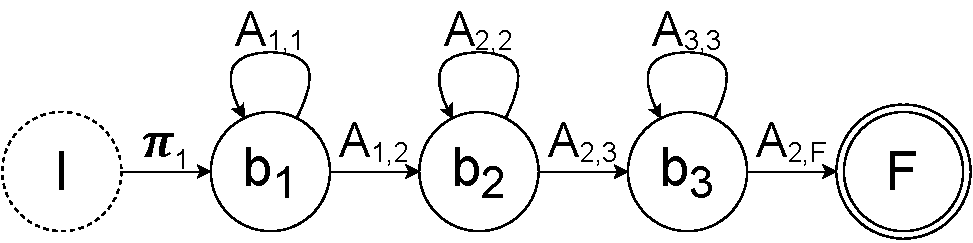
\includegraphics[width=0.55\textwidth]{figuras/estructura_hmm.pdf}
\caption{Representació d'un HMM. Podem apreciar els tres estats $b_1$, $b_2$ i $b_3$ que representen l'inici, la part central i el final del fonema. També s'observen els estats Inicial i Final, que indiquen quan ha començat i acabat el reconeixement del fonema en qüestió.}
\label{fig:estructura_hmm}
\end{figure}

Per tant, la probabilitat que el model HMM associat a un fonema $f$ genere o explique la seqüència acústica $\textbf{x}$ és:

\begin{equation}
    P_f(\textbf{x}) = \sum_{q \in Q} \prod_{t=1}^{|q|} P(q_t|q_{t-1}) P(\textbf{x}_t|q_t)
    \label{eq:hmm_prob}
\end{equation}
on $q_t$ és el $t$-èsim estat assolit per la seqüència d'estats $q$, $\textbf{x}_t$ és $t$-èsim vector de la seqüència de vectors $\textbf{x}$, $P(q_t|q_{t-1})$ és la probabilitat de transitar d'un estat $q_{t-1}$ a un estat $q_t$, i $P(\textbf{x}_t|q_t)$ és la probabilitat d'emissió del vector $\textbf{x}_t$ a l'estat $q_t$.

Pel que fa a les probabilitats d'emissió, $P(\textbf{x}_t|q_t)$, tradicionalment s'han modelat mitjançant mixtures de Gaussianes (GMMs)~\ref{cap02_mixtures}, entrenades amb l'algorisme Expectation-Maximization (EM). En aquest cas, parlem de models acústics basats en GMM-HMMs.

Aquests models acústics, quan són acoblats juntament amb el model del llenguatge a un sistema ASR, ajunten els estats Inicial i Final de fonemes ($P_f(\textbf{x})$ o, equivalentment, $P(\textbf{x}|f)$) o trifonemes consecutius. Ho fan d'acord amb la informació proporcionada per diccionaris de pronunciació fonètics (model lèxic), per a conformar HMMs a nivell de paraula: $P_w(\textbf{x})$, o directament, $P(\textbf{x}|w)$, el model acústic pròpiament dit. 

Més recentment, en l'última dècada, les xarxes neuronals, gràcies al seu gran poder discriminatiu, han reemplaçat els GMMs en el modelat de les probabilitat d'emissió. 
Açò va permetre generar models més robusts, ja que no fan cap assumpció sobre l'origen de les dades, que també permeten obtenir uns resultats significativament millors\cite{hinton2012}. 
Per tal de poder explotar el potencial de les DNNs en l'estimació de les probabilitats d'emissió, $P(\textbf{x}_t|q_t)$, primer s'aplica el teorema de Bayes sobre l'equació~\ref{eq:hmm_prob}:

\begin{equation}
P_f(\textbf{x}) = \sum_{q \in Q} \prod_{t=1}^{|q|} P(q_t|q_{t-1}) \frac{P(\textbf{x}_t) P(q_t|\textbf{x}_t)}{P(q_t)} 
\end{equation}

A continuació, considerant l'equivalència formal dels HMMs a nivell de fonema $P_f(\textbf{x})$, amb els HMMs a nivell de paraula $P_w(\textbf{x})$ o $P(\textbf{x}|w)$, així com que, en la cerca, s'aplica l'aproximació de Viterbi per obtenir el camí $q$ més probable, podem reescriure l'equació~\ref{eq:form_argmax_classif_ASR} com segueix:

\begin{equation}
	\hat{w} = \argmax_{w \in L^{*}} P(w | \textbf{x}) = \argmax_{w \in L^{*}} \max_{q \in Q} \prod_{t=1}^{|q|} P(q_t|q_{t-1}) \frac{P(\textbf{x}_t) P(q_t|\textbf{x}_t)}{P(q_t)} \, P(w)
    \label{eq:cerca_nivell_paraules}
\end{equation}

A l'igual que en el pas de l'equació~\ref{eq:form_argmax_classif} a l'equació~\ref{eq:form_argmax_classif_simpli}, tenim que $P(\textbf{x}_t)$ és constant i independent de la classe de l'objecte, raó per la qual podem obviar-la i estalviar-nos calcular-la. Pel que fa a $P(q_t)$, les probabilitats a priori dels estats HMM, poden calcular-se mitjançant l'aprenentatge amb dades d'entrenament i normalitzant els comptes de cada estat $q_t$ durant aquest entrenament.
%Alguns dels actuals sistemes estat de la tècnica gasten dues aproximacions per a estimar $P(q_t|x_t)$, i conseqüentment, les probabilitats d'emissió:
Per últim, $P(q_t|\textbf{x}_t)$, i conseqüentment, les probabilitats d'emissió del HMM integrat, poden ser modelades per xarxes neuronals de tipus FF-DNN (models FF-DNN-HMM)~\cite{hinton2012}, Convolucionals (models CNN-HMM)~\cite{6857341}, BLSTM (models BLSTM-HMM)~\cite{mllp2020} o Transformer (models T-HMM)~\cite{wang2020transformers_asr}.

Aquest treball se centra en el desenvolupament d'un sistema ASR híbrid BLSTM-HMM, tecnologia que encara demostra estar a la avantguarda de la tècnica~\cite{jorge2021iberspeech}.
La lectora pot trobar més informació sobre els models ocults de Markov a l'àmbit del ASR a \cite[capítol 8.4]{jurafskySLP}.



\subsection{Preprocés i extracció de característiques}
\label{cap02_preprocessat_acustic}
El primer pas que cal donar per a construir models acústics és el preprocès i l'extracció de característiques de les dades d'entrenament per tal d'obtenir els vectors de característiques $\textbf{x}$. 

En primer lloc, cal obtenir la versió digital de l'ona acústica. Aquesta conversió es divideix en dues tasques: d'una banda, cal realitzar un mostreig, consistent en mesurar l'amplitud de l'ona en un instant particular de temps.
Seran necessàries un mínim de dues mostres per cada cicle de l'ona (una per a la part positiva de l'ona i l'altra per a la negativa). A major quantitat de mostres, major qualitat, però tenint en compte que la màxima freqüència que podem mesurar és la meitat de la freqüència de mostreig (freqüència de Nyquist\cite{grenander1959probability}).
Per a l'ASR és suficient amb mostres de 16 KHz, ja que els principals sons de la fonologia humana es troben baix de l'espectre dels 8 KHz.
Per altra banda, cal quantificar la informació, codificant el valor de cada amplitud mesurada, típicament, en nombres enters de 16 bits.

A continuació es generen una sèrie de finestres temporals de les quals s'extrauen els vectors de característiques. En aquestes finestres cal fixar tres paràmetres: la mida de la finestra (en ms), el retard entre una finestra i la seua adjacent (en ms), i la forma de la finestra.
La figura~\ref{fig:finestres_temporals} representa el procés de generar diverses finestres per a poder extraure vectors de característiques.
\begin{figure}[ht!]
    \centering
    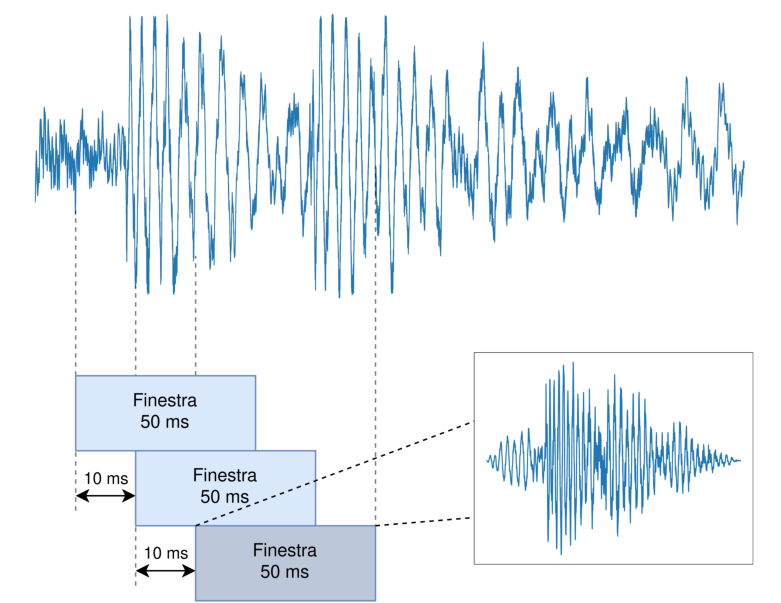
\includegraphics{figuras/finestres_temporals.pdf}
    \caption{Finestres amb forma de Hamming de 50 ms amb un retard de 10 ms.}
    \label{fig:finestres_temporals}
\end{figure}
Típicament, s'usen finestres de Hamming, ja que la finestra rectangular talla l'àudio de forma abrupta. Açò és resol atenuant ambdós costats de la finestra segons la fórmula:

        \begin{align}
            w(n)_{Rectangular} &=
                \begin{dcases}
                    1 & 0 \leq n \leq L-1 \\
                    0 & \text{altre cas}
                \end{dcases} \\
            w(n)_{Hamming} &=
                \begin{dcases}
                    0.54 - 0.46 \cos \frac{2 \pi n}{L} & 0 \leq n \leq L-1 \\
                    0 & \text{altre cas}
                \end{dcases}
        \end{align}
        A la figura~\ref{fig:comparativa_finestres} s'aprecia la diferència d'ambdues formes.

        \begin{figure}[!ht]
             \centering
             \begin{subfigure}{0.4\textwidth}
                 \centering
                 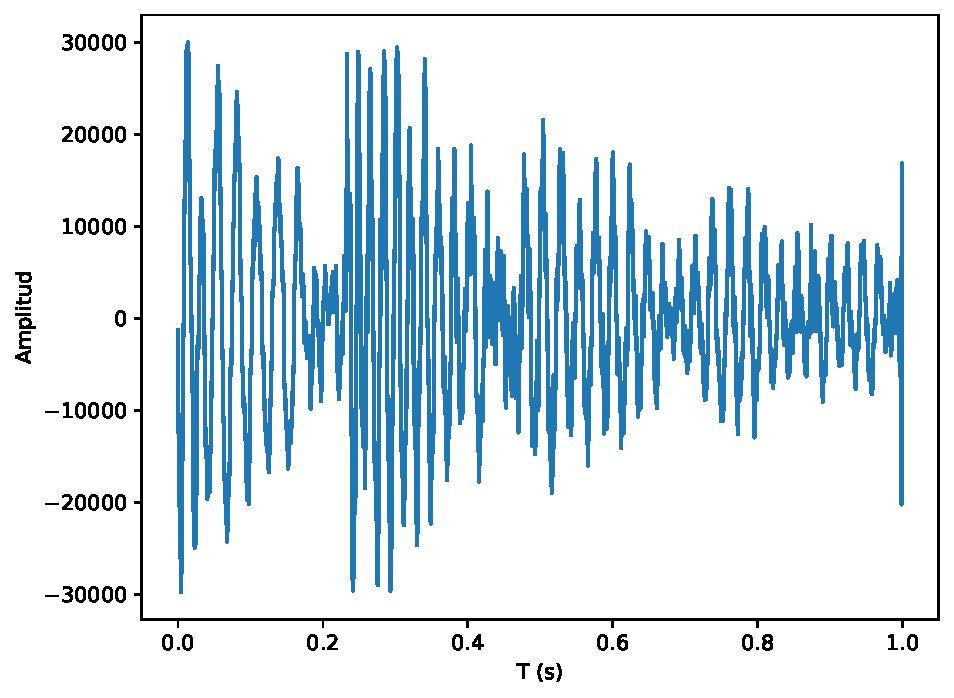
\includegraphics[width=\textwidth]{figuras/finestra_rect.pdf}
                 \caption{Finestra rectangular}
             \end{subfigure}
             \begin{subfigure}{0.4\textwidth}
                 \centering
                 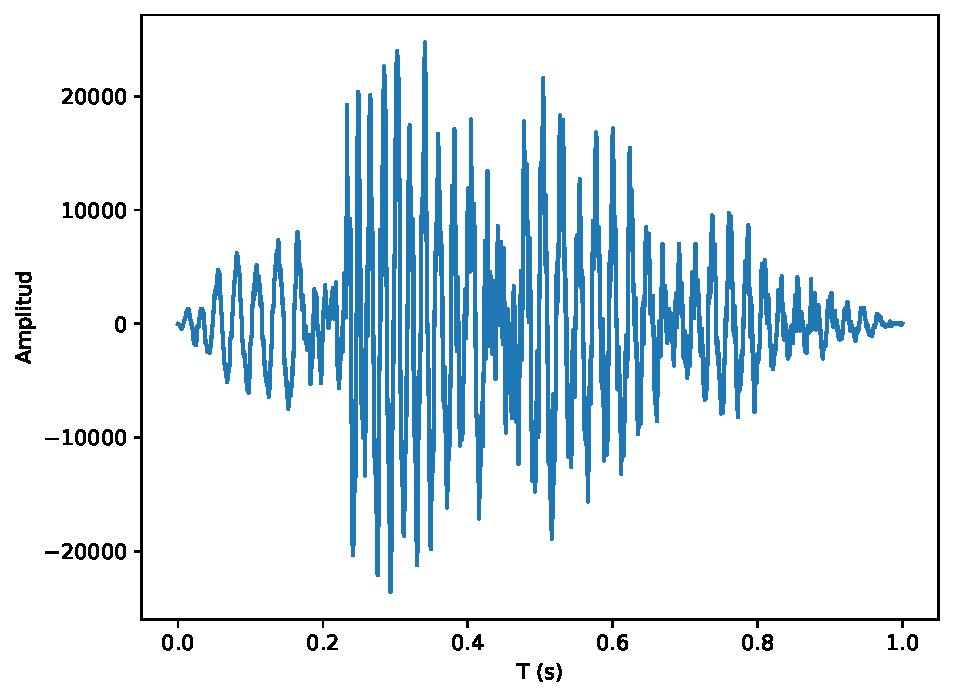
\includegraphics[width=\textwidth]{figuras/finestra_hamm.pdf}
                 \caption{Finestra de Hamming}
             \end{subfigure}
             \caption{Comparativa de la mateixa mostra acústica baix les dues formes de finestra. S'observa l'atenuament en els extrems de la finestra de Hamming.}
             \label{fig:comparativa_finestres}
        \end{figure}



El següent pas és extraure la informació de cada finestra. Es realitza una transformada discreta de Fourier (Discrete Fourier Transform, DFT), que extrau l'energia del senyal en diferents bandes de freqüència. Aquesta transformada es defineix com:

    \begin{equation}
        X_k = \sum_{n=0}^{N-1} x_n \cdot e^{- \frac{2 \pi i}{N} kn} \quad  \forall k \in{0, \dots, N-1},
    \end{equation}
    on $i$ és la unitat imaginaria i $e^{- \frac{2 \pi i}{N}}$ és l'N-ésima arrel de la unitat.

Típicament, s'usa l'algorisme de \textit{transformada ràpida de Fourier} (\textit{FFT, Fast Fourier Transform}) per a calcular la \textit{DFT}. Aquesta implementació es molt eficient, però solament funciona per a valors de $N$ que siguen potències de 2.
    Per a més informació sobre la transformada discreta de Fourier, es recomana a la lectora~\cite{mathews2012complex}.

En quart lloc, degut a que l'oïda humana no percep de la mateixa manera totes les bandes, és molt més sensible a freqüències baixes que a altes, cal modelar aquesta percepció per millora notablement la qualitat del reconeixement de la parla. S'assoleix mitjançant un banc de filtres Mel~\cite{8732232}.
El nombre de dimensions del vector resultant és igual al nombre de filtres que formen el banc. La figura~\ref{fig:mel_filterbank} exemplifica un banc de filtres triangulars que implementen aquesta idea.

    \begin{figure}[ht!]
        \centering
        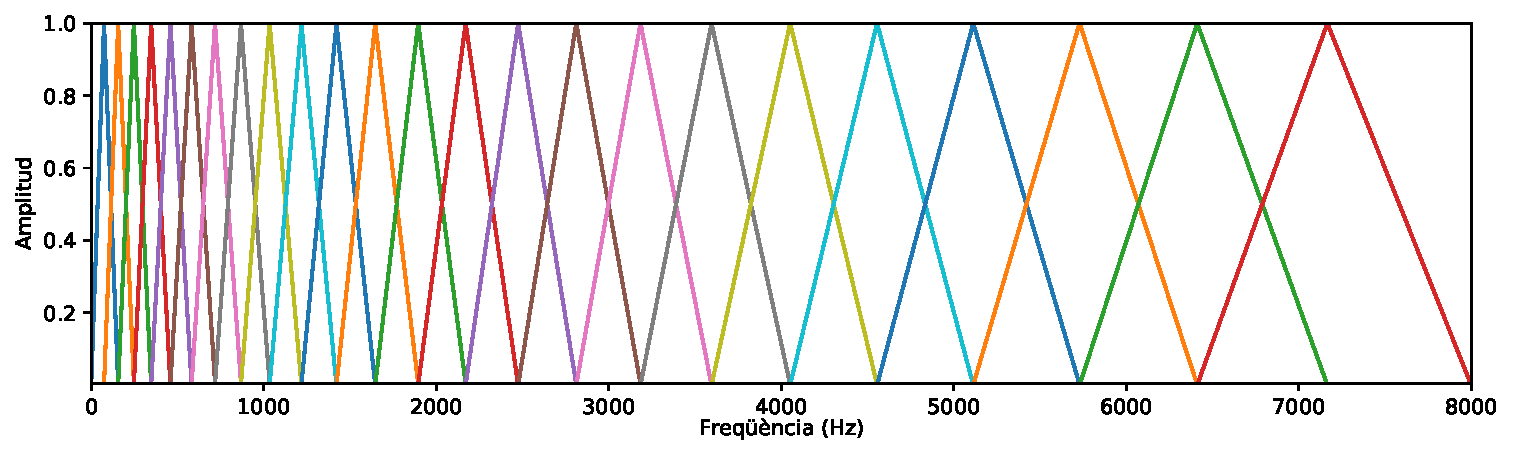
\includegraphics[width=\textwidth]{figuras/mel_filterbank.pdf}
        \caption{Banc de filtres Mel. Cada filtre triangular està espaiat logarítmicament mitjançant l'escala mel.}
        \label{fig:mel_filterbank}
    \end{figure}
A l'eixida d'aquest pas, tenim els vectors de característiques Filterbanks. 
A continuació s'aplica l'algorisme de \textit{transformada cosinus discreta} (\textit{DCT, Discrete Cosine Transform}) i, finalment, es normalitzen les mostres amb l'objectiu de minimitzar les seues diferències. D'aquesta manera xicotetes diferències en la pronunciació i la sonoritat perden rellevància, augmentant la capacitat de generalització del model.
L'eixida d'aquest preprocès són els vectors de característiques MFCC (Mel Frequency Cepstral Coefficient), un per cada frame.



\subsection{Modelat del llenguatge}
\label{cap02_asr_lm}

El model del llenguatge és l'altre component principal del sistema híbrid que representa l'estructura pròpia del llenguatge modelant $P(w)$. En altres paraules, calcula la probabilitat que una paraula $w_i$ aparega donada una història o context previ $w_1, w_2, \dots, w_{i-1}$.
El fet que els models del llenguatge s'entrenen amb dades de text monolingüe (molt abundants i de fàcil accés), ens permet entrenar models robusts i potents. De fet, aquest és el principal motiu que ens fa optar per una aproximació híbrida i que assoleix que ara mateix siga l'aproximació més puntera enfront dels sistemes end-to-end.

Existeixen diferents aproximacions al modelat de llenguatge. Tradicionalment, s'ha emprat l'aproximació estadística basada en comptes, representada pels models de n-grames: seqüències contigues d'$n$ paraules a les quals se solen referir pel nombre d'aquestes (unigrama, bigrama, trigrama, etc.). El model del llenguatge utilitzat al sistema final empra n-grames per a aproximar $P(w)$ com la probabilitat d'una paraula $w_i$ donada una història $h_i=w_1 w_2 \dots w_{i-1}$ (seqüència prèvia de paraules). Pot expressar-se mitjançant la probabilitat condicional com $P(w_i|h_i)$, o formalment:

\begin{equation}
P(w) \approx \prod_{i=1}^{I+1} P(w_i|w_{\max(i - n + 1, \ 0)}^{i-1})
\end{equation}
on I es la grandària de $w$, $n$ la mida de l'n-grama, $w_i^{i+j}$ representa la seqüència de paraules $(w_i, w_{i+1}, \dots, w_j) \in w$, i $w_0$ i $w_{I+1}$, sengles estats especials que representen els \textit{tokens} especials d'inici i final de frase. D'aquesta manera, un n-grama de segon ordre o bigrama, permet contextualitzar únicament la paraula anterior a l'actual i un trigrama les dues anteriors. Per exemple, en la frase \guillemotleft Llança el dau de vint cares\guillemotright, la probabilitat que la paraula \guillemotleft cares\guillemotright ~aparega després de la paraula \guillemotleft vint\guillemotright ~pot expressar-se amb un model trigrama com:

\begin{align}
    P( \text{ \guillemotleft de vint cares\guillemotright } ) = 
    &P( \text{ \guillemotleft de\guillemotright } | \text{ IDF } ) \nonumber \\
    &P( 
        \text{ \guillemotleft vint\guillemotright } | 
        \text{ IDF}, \text{ \guillemotleft de\guillemotright } 
    )  \\
    &P(
        \text{ \guillemotleft cares\guillemotright } | 
        \text{ \guillemotleft de vint\guillemotright }
    )  \nonumber \\
    &P(
        \text{ FDF } | 
        \text{ \guillemotleft vint cares\guillemotright }
    ) \nonumber
\end{align}
on $IDF$ i $FDF$ són els tokens especials de \guillemotleft Inici de frase\guillemotright ~i \guillemotleft Final de frase\guillemotright. 

Més recentment, els models de llenguatge continus o neuronals, s'han imposat clarament als models de n-grames, especialment els basats en mecanismes d'autoatenció~\cite{wang2019transformers_lm, baqueroarnal20_interspeech}, com l'arquitectura Transformer, exhibint una capacitat d'atenció potencialment infinita a qualsevol paraula de la història prèvia, en clar contrast amb les severes limitacions dels n-grames, que sols retenen una història de $n-1$ paraules, i on típicament $n \leq 4$.
%L'aplicació de l'arquitectura transformer al model del llenguatge ha assolit millors resultats que els anteriors models estats de la tècnica~\cite{wang2019transformers_lm}~\cite{baqueroarnal20_interspeech}.

En aquest treball s'utilitzaran models de llenguatge de n-grames i Transformer proporcionats per investigadors del grup de recerca MLLP, per aquesta raó, el seu entrenament i la seua optimització queda fora de l'abast d'aquest treball.

\subsection{Descodificació / Reconeixement}
\label{cap02_asr_decoder}

La descodificació és l'etapa en la qual ambdós models, l'acústic i el del llenguatge, es combinen per a trobar la seqüència de paraules més probable per a la mostra acústica donada d'acord amb l'equació~\ref{eq:cerca_nivell_paraules}. Per a fer-ho es genera un multigraf dirigit amb totes les paraules del vocabulari, sent cada node, un fonema de la paraula. Una simplificació d'aquesta estructura pot observar-se a la Figura~\ref{fig:decoder_simpli}.

\begin{figure}[ht!]
\centering
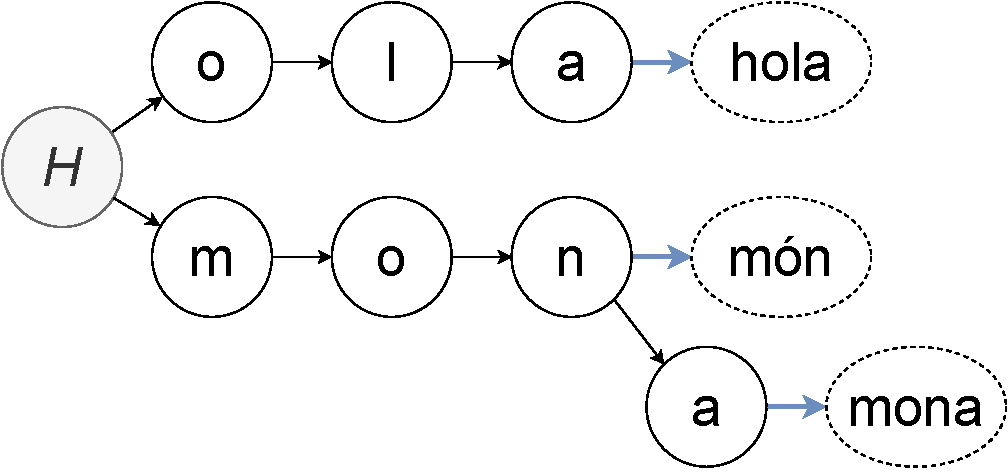
\includegraphics[width=0.5\textwidth]{figuras/espai_cerca.pdf}
\caption{Exemple d'un graf de cerca capaç de reconéixer una paraula. Per motius de brevetat es considera un vocabulari de solament tres paraules: \guillemotleft hola\guillemotright, \guillemotleft món\guillemotright i \guillemotleft mona\guillemotright. L'estat inicial, $H$, denota la història actual. En concret, les fletxes blaves indiquen l'instant exacte en el qual està calculada la probabilitat d'una paraula, que comporta realitzar una consulta explícita al model de llenguatge, per exemple \guillemotleft hola\guillemotright, donada la història, $P(paraula | H)$.}
\label{fig:decoder_simpli}
\end{figure}

S'ha de tindre en compte que l'espai de cerca és, en qualsevol cas, molt gran, ja que totes les paraules del vocabulari del sistema són assolibles des de qualsevol història. A més, durant la descodificació, aquestes decisions es prenen a escala de frame. Aquest mecanisme posa en compromís la latència del sistema i pot no servir per a tasques d'ASR en temps real.

Una solució parcial és aplicar tècniques de poda de l'espai de cerca, de tipus beam-search, que solament mantinguen un subgrup d'hipòtesis més probables en cada instant. Però presenta un altre inconvenient: una hipòtesi descartada pot ser realment més encertada que una que es mantén, ja que durant la cerca, solament es té en compte l'opinió del model acústic, mentre que el model de llenguatge sols aporta el seu coneixement quan el procés de descodificació transita d'un estat fonema a un estat paraula.
Per solucionar-ho, s'usen taules estàtiques de look-ahead~\cite{jorge19_interspeech}, un algorisme recursiu que, des de les fulles de la cerca (totes les paraules del vocabulari), va assignant a cada estat la màxima probabilitat assolible des d'ell, segons el model del llenguatge. D'aquesta manera, durant la cerca, quan hi ha una bifurcació solament cal restar a l'estat actual la probabilitat actual màxima del LM i sumar la màxima assolible per cada camí. 
D'aquesta manera, durant la cerca, totes les hipòtesis tenen també informació aportada pel model del llenguatge i la quantitat de consultes que se li realitzen es redueix dràsticament.

\subsection{Avaluació de sistemes ASR}
\label{cap02_asr_avaluacio}

Els sistemes ASR s'avaluen de forma objectiva mitjançant la taxa d'error per paraula (WER, Word Error Rate), que es defineix com la mínima distància entre les transcripcions obtingudes pel sistema i les originals, utilitzant les dades de \textit{development} i \textit{test}.
Aquesta mètrica és similar a la distància de Levenshtein: permet insercions, substitucions i eliminacions a escala de paraula. Es defineix com:

\begin{equation}
WER = \frac{I + S + E}{R}\cdot 100
\end{equation}
on $I$, $S$ i $E$ són, respectivament, el nombre d'insercions, substitucions i eliminacions necessàries perquè la nostra transcripció siga idèntica a l'original, i $R$ és el total de paraules de la transcripció.
El WER pot entendres, de forma intuïtiva, com el percentatge de paraules de la transcripció automàtica que cal esmentar per a obtenir la transcripció correcta de referència.

No obstant això, els components principals dels sistemes ASR, això és, el model acústic i el model del llenguatge, estan desenvolupats i optimitzats de forma independent i amb diferents fonts de dades. Per tant, durant l'etapa de desenvolupament del sistema ASR, el seu rendiment individual es mesura utilitzant altres mètriques. 
En el cas dels models acústics basats en xarxes neuronals, aquests estan entrenats minimitzant la taxa d'error de classificació de frames (FER, Frame Error Rate) en un conjunt de desenvolupament donat.
FER està definida com el nombre de frames incorrectament classificats dividit entre el total de frames analitzats:

\begin{equation}
FER = \frac{F_{\text{incorrectes}}}{F_{\text{totals}}}
\end{equation}

